\documentclass[a4paper,10pt,twocolumn]{article}
\usepackage[english]{babel}
\usepackage[style=ieee,backend=bibtex]{biblatex} \bibliography{ref.bib}
\usepackage[hidelinks]{hyperref}
\usepackage{fancyhdr}
\usepackage{float}
\usepackage{graphicx}
\usepackage[latin1]{inputenc}
\usepackage{nomencl}
\usepackage{multicol}
\usepackage{siunitx}
\usepackage{tikz}
    \usetikzlibrary{arrows}
    \usetikzlibrary{patterns}
    \usetikzlibrary{3d}
\usepackage{titling}
\usepackage{xspace}

\newcommand{\Comsol}{\textsc{Comsol}\xspace}
\newcommand{\comsol}{\textsc{comsol}\xspace}
\newcommand{\Cmos}{\textsc{Cmos}\xspace}
\newcommand{\cmos}{\textsc{cmos}\xspace}
\newcommand{\Mems}{\textsc{Mems}\xspace}
\newcommand{\mems}{\textsc{mems}\xspace}

% Top matter
\title{\Mems Multimorph Temperature Sensors in
    \Comsol~Multiphysics\textsuperscript{\textregistered}}
\author{Z0966990}
\date{\today}

% Headers and footers
\pagestyle{fancy}
\fancyhf{}
\lhead{
\includegraphics[width=0.1\textwidth]{img/Durham.png}}
\chead{\thetitle}
\rhead{\theauthor}
\cfoot{\thepage}

\begin{document}

% Title and abstract
\thispagestyle{plain}

\twocolumn[{
\begin{@twocolumnfalse} \centering
    
\includegraphics[width=0.2\textwidth]{img/Durham.png}\\
    \Large\thetitle
    \vskip0.2em
    \large Level 3 Semiconductor, Physics and Devices\\
    \vskip0.4em
    \large\theauthor\\
    \vskip0.4em
    \large\thedate\\
    \hrulefill
    \renewcommand{\abstractname}{\large Abstract}
    \begin{abstract}
        In this report it is detailed how
    \end{abstract}
    \vskip\parsep
\end{@twocolumnfalse}
}]


\makenomenclature

% Acronyms
\nomenclature[A0]{\mems}{Microelectromechanical systems}

\printnomenclature

\begin{figure}[h]
    \centering
    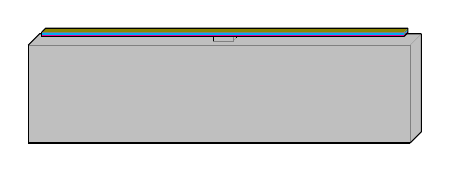
\begin{tikzpicture}[scale=0.4\textwidth/0.780cm]
        % Substrate faces
        \begin{scope}[canvas is yz plane at x=0.780]
            \path [fill=lightgray] (0,0) rectangle (0.200,0.060);
        \end{scope}
        \begin{scope}[canvas is zx plane at y=0.200]
            \path [fill=lightgray] (0,0) rectangle (0.060,0.780);
        \end{scope}
        \begin{scope}[canvas is xy plane at z=0.060]
            \path [fill=lightgray] (0,0) rectangle (0.780,0.200);
        \end{scope}

        % Substrate internal edges
        \begin{scope}[canvas is yz plane at x=0.780]
            \draw [gray,ultra thin] (0.200,0.000) -- (0.200,0.060);
        \end{scope}
        \begin{scope}[canvas is zx plane at y=0.200]
            \draw [gray,ultra thin] (0.060,0.000) -- (0.060,0.780);
        \end{scope}
        \begin{scope}[canvas is xy plane at z=0.060]
            \draw [gray,ultra thin] (0.780,0.000) -- (0.780,0.200);
        \end{scope}

        % Substrate external edges
        \begin{scope}[canvas is yz plane at x=0.780]
            \draw [thin] (0.000,0.060) -- (0.000,0.000) -- (0.200,0.000);
        \end{scope}
        \begin{scope}[canvas is zx plane at y=0.200]
            \draw [thin] (0.000,0.780) -- (0.000,0.000) -- (0.060,0.000);
        \end{scope}
        \begin{scope}[canvas is xy plane at z=0.060]
            \draw [thin] (0.000,0.200) -- (0.000,0.000) -- (0.780,0.000);
        \end{scope}

        % Pillar faces
        \begin{scope}[canvas is yz plane at x=0.410]
            \path [fill=lightgray] (0.200,0.020) rectangle (0.210,0.040);
        \end{scope}
        \begin{scope}[canvas is xy plane at z=0.040]
            \path [fill=lightgray] (0.370,0.200) rectangle (0.410,0.210);
        \end{scope}

        % Pillar internal edges
        \begin{scope}[canvas is yz plane at x=0.410]
            \draw [gray,ultra thin] (0.200,0.020) -- (0.200,0.040);
        \end{scope}
        \begin{scope}[canvas is xy plane at z=0.040]
            \draw [gray,ultra thin] (0.370,0.200) -- (0.410,0.200) --
                (0.410,0.210);
        \end{scope}

        % Pillar external edges
        \begin{scope}[canvas is yz plane at x=0.370]
            \draw [thin] (0.200,0.040) -- (0.210,0.040);
        \end{scope}
        \begin{scope}[canvas is yz plane at x=0.410]
            \draw [thin] (0.200,0.020) -- (0.210,0.020);
        \end{scope}

        % Layers faces
        \begin{scope}[canvas is yz plane at x=0.760]
            \path [fill=olive] (0.216,0.020) rectangle (0.219,0.040);
            \path [fill=cyan] (0.213,0.020) rectangle (0.216,0.040);
            \path [fill=magenta] (0.210,0.020) rectangle (0.213,0.040);
        \end{scope}
        \begin{scope}[canvas is zx plane at y=0.219]
            \path [fill=olive] (0.020,0.020) rectangle (0.040,0.760);
        \end{scope}
        \begin{scope}[canvas is xy plane at z=0.040]
            \path [fill=olive] (0.020,0.216) rectangle (0.760,0.219);
            \path [fill=cyan] (0.020,0.213) rectangle (0.760,0.216);
            \path [fill=magenta] (0.020,0.210) rectangle (0.760,0.213);
        \end{scope}

        % Layers internal edges
        \begin{scope}[canvas is yz plane at x=0.760]
            \draw [gray,ultra thin] (0.219,0.020) -- (0.219,0.040);
        \end{scope}
        \begin{scope}[canvas is zx plane at y=0.219]
            \draw [gray,ultra thin] (0.040,0.020) -- (0.040,0.760);
        \end{scope}
        \begin{scope}[canvas is xy plane at z=0.040]
            \draw [gray,ultra thin] (0.760,0.210) -- (0.760,0.219);
        \end{scope}

        % Layers external edges
        \begin{scope}[canvas is yz plane at x=0.760]
            \draw [thin] (0.219,0.020) -- (0.210,0.020) -- (0.210,0.040);
        \end{scope}
        \begin{scope}[canvas is zx plane at y=0.219]
            \draw [thin] (0.020,0.760) -- (0.020,0.020) -- (0.040,0.020);
        \end{scope}
        \begin{scope}[canvas is xy plane at z=0.040]
            \draw [thin] (0.020,0.219) -- (0.020,0.210) -- (0.760,0.210);
        \end{scope}



    \end{tikzpicture}
\end{figure}

\begin{figure}[h]
    \centering
    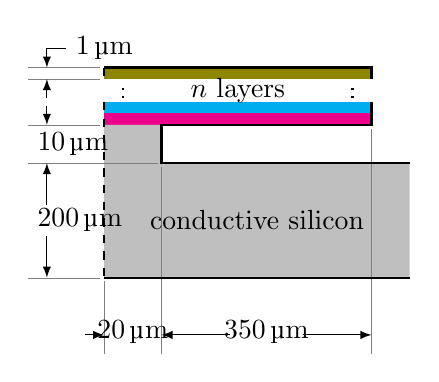
\begin{tikzpicture}[scale=0.4\textwidth/1cm]
        % Layers
        \path [fill=olive]   (0.20,0.72) rectangle (0.90,0.75);
        \draw [dotted,thick] (0.85,0.67) -- (0.85,0.71);
        \draw [dotted,thick] (0.25,0.67) -- (0.25,0.71);
        \path [fill=cyan]    (0.20,0.63) rectangle (0.90,0.66);
        \path [fill=magenta] (0.20,0.60) rectangle (0.90,0.63);
        \path [fill=lightgray] (0.20,0.20) -- (1.00,0.20) -- (1.00,0.50) -- 
            (0.35,0.50) -- (0.35,0.60) -- (0.20,0.60) -- (0.20,0.20);
        
        % Witness lines
        \draw [gray,ultra thin] (0.00,0.75) -- (0.19,0.75);
        \draw [gray,ultra thin] (0.00,0.72) -- (0.19,0.72);
        \draw [gray,ultra thin] (0.00,0.60) -- (0.19,0.60);
        \draw [gray,ultra thin] (0.00,0.50) -- (0.34,0.50);
        \draw [gray,ultra thin] (0.00,0.20) -- (0.19,0.20);

        \draw [gray,ultra thin] (0.20,0.00) -- (0.20,0.19);
        \draw [gray,ultra thin] (0.35,0.00) -- (0.35,0.49);
        \draw [gray,ultra thin] (0.90,0.00) -- (0.90,0.59);

        % Outline
        \draw [thick] (0.20,0.20) -- (1.00,0.20);
        \draw [thick] (1.00,0.50) -- (0.35,0.50) -- (0.35,0.60) -- (0.90,0.60)
            -- (0.90,0.66);
        \draw [thick] (0.90,0.72) -- (0.90,0.75) -- (0.20,0.75);
        \draw [dashed,thick] (0.20,0.75) -- (0.20,0.72);
        \draw [dashed,thick] (0.20,0.66) -- (0.20,0.20);

        % Labels
        \node at (0.55,0.69) {$n$ layers};
        \node [align=center] at (0.60,0.35) {conductive silicon};

        % Dimensions
        \node [right] at (0.10,0.80) {\SI{1}{\micro\meter}};
        \draw [latex-] (0.05,0.75) -- (0.05,0.80) -- (0.10,0.80);
        \draw [-latex] (0.05,0.67) -- (0.05,0.72);
        \draw [latex-] (0.05,0.60) -- (0.05,0.65);
        \node [right] at (0.00,0.55) {\SI{10}{\micro\meter}};
        \draw [-latex] (0.05,0.39) -- (0.05,0.50);
        \node [right] at (0.00,0.35) {\SI{200}{\micro\meter}};
        \draw [latex-] (0.05,0.20) -- (0.05,0.31);

        \draw [-latex] (0.15,0.05) -- (0.20,0.05);
        \node [above] at (0.275,0.00) {\SI{20}{\micro\meter}};
        \draw [latex-] (0.35,0.05) -- (0.53,0.05);
        \node [above] at (0.625,0.00) {\SI{350}{\micro\meter}};
        \draw [-latex] (0.72,0.05) -- (0.90,0.05);
    \end{tikzpicture}
    \caption{Multimorph temperature sensor model---not to scale.}
    \label{fig:model}
\end{figure}

\printbibliography

\end{document}